\chapter{Membangun Model Prediksi}

Untuk pratikum saati ini menggunakan buku \textit{Python Artificial Intelligence Projects for Beginners}\cite{eckroth2018python}. Dengan praktek menggunakan python 3 dan editor anaconda dan library python scikit-learn.
Dataset ada di https://github.com/PacktPublishing/Python-Artificial-Intelligence-Projects-for-Beginners .
Tujuan pembelajaran pada pertemuan pertama antara lain:
\begin{enumerate}
\item
Mengerti implementasi klasifikasi
\item
Memahami data set, training dan testing data
\item
Memahami Decission tree.
\item
Memahami information gain dan entropi.
\end{enumerate}
Tugas dengan cara dikumpulkan dengan pull request ke github dengan menggunakan latex pada repo yang dibuat oleh asisten riset. Kode program menggunakan input listing ditaruh di folder src ekstensi .py dan dipanggil ke latex dengan input listings. Tulisan dan kode tidak boleh plagiat, menggunakan bahasa indonesia yang sesuai dengan gaya bahasa buku teks.

\section{Teori}
Praktek teori penunjang yang dikerjakan(nilai 5 per nomor, untuk hari pertama) :
\begin{enumerate}
\item
Jelaskan apa itu binary classification dilengkapi ilustrasi gambar sendiri.
\newline Jawab:
\newline Binary classification merupakan proses pengklasifikasian elemen-elemen himpunan berdasarkan aturan klasifikasi yang ouputnya dibagi menjadi 2 kelompok.

\item
Jelaskan apa itu supervised learning dan unsupervised learning dan clustering dengan ilustrasi gambar sendiri.
\newline Jawab:
\newline Supervised Learning merupakan sebuah pendekatan yang ditentukan berdasarkan penggunaan
traning dataset yang berlabel/labeled dataset dan digunakan untuk melakukan klasifikasi data atau memprediksi hasil secara akurat.
\newline Unsupervised Learning merupakan sebuah pendekatan yang ditentukan berdasarkan penggunaan
traning dataset yang tidak berlabel dan digunakan untuk menganalisa serta mengelompokan kumpulan data yang tidak berlabel.
\newline Clustering merupakan sebuah proses pengelompokan data ke dalam beberapa cluster yang dimana data-data di suatu cluster tersebut memiliki kemiripan.

\item
Jelaskan apa itu evaluasi dan akurasi dari buku dan disertai ilustrasi contoh dengan gambar sendiri.
\newline Jawab:
\newline Evaluasi merupakan kegiatan untuk mengukur sebarapa baik nilai performa dari suatu
model dengan cara mengukur akurasinya. 
\newline Akurasi merupakan tigkat ketepatan yang diklasifikasikan dengan benar dari suatu model.

\item
Jelaskan bagaimana cara membuat dan membaca confusion matrix, buat confusion matrix buatan sendiri.
\newline Jawab:
\newline Cara membuat dan membaca confusion matrix:
\begin{enumerate}
	\item Menentukan studi kasusnya.
	\item Membuat ke dalam Decision Tree.
	\item Menyiapkan data testing.
	\item Mencari value dari variabel, misalnya yaitu a,b,c,d.
	\item Mencari value dari recall, precision, accuracy, dan error state.
\end{enumerate}

\item
Jelaskan bagaimana K-fold cross validation bekerja dengan gambar ilustrasi contoh buatan sendiri.
\newline Jawab:
\newline Cara kerja dari K-fold cross validation:
\begin{enumerate}
	\item Mengacak dataset secara random.
	\item Membagi dataset tersebut kedalam k-group, yaitu sebagai test dataset dan sisanya sebagai training dataset.
	\item Memasang model pada training set dan evaluasi pada test dataset.
	\item Menyimpan skor evaluasi dan buang modelnya.
	\item Meringkas keterampilan model menggunakan sampel skor menggunakan	model evaluasi.
\end{enumerate}

\item
Jelaskan apa itu decision tree dengan gambar ilustrasi contoh buatan sendiri.
\newline Jawab:
\newline Decision Tree merupakan suatu metode yang digunakan untuk membatu dalam pengambilan keputusan dengan menggunakan model pohon.

\item
Jelaskan apa itu information gain dan entropi dengan gambar ilustrasi buatan sendiri.
\newline Jawab:
\newline Information gain merupakan kumpulan informasi yang didapatkan dari variable acak.
\newline Entropi merupakan tingkat keacakan pada informasi yang diperloh dari information gain dan sedang diproses.

\end{enumerate}

\newpage
\section{scikit-learn}
Dataset ambil di https://github.com/PacktPublishing/Python-Artificial-Intelligence-Projects-for-Beginners folder Chapter01.
Tugas anda adalah, dataset ganti menggunakan \textbf{student-mat.csv} dan mengganti semua nama variabel dari kode di bawah ini dengan nama-nama makanan (NPM mod 3=0), kota (NPM mod 3=1), buah (NPM mod 3=2), . Jalankan satu per satu kode tersebut di spyder dengan menggunakan textit{Run current cell}. Kemudian Jelaskan dengan menggunakan bahasa yang mudah dimengerti dan bebas plagiat dan wajib skrinsut dari komputer sendiri masing masing nomor di bawah ini(nilai 5 masing masing pada hari kedua).

\begin{enumerate}

\item
\begin{verbatim}
	# load dataset (student mat pakenya)
	import pandas as pd
	d = pd.read_csv('student-mat.csv', sep=';')
	len(d)
\end{verbatim}
\newline Output: 
\begin{figure}[!htbp]
	\centering
	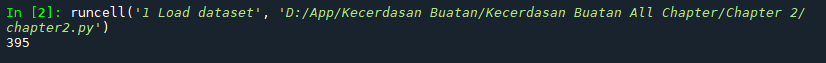
\includegraphics[scale=0.5]{figures/chapter2/1.PNG}
\end{figure}

\item
\begin{verbatim}
	# generate binary label (pass/fail) based on G1+G2+G3 
	# (test grades, each 0-20 pts); threshold for passing is sum>=30
	d['pass'] = d.apply(lambda row: 1 if (row['G1']+row['G2']+row['G3']) 
											>= 35 else 0, axis=1)
	d = d.drop(['G1', 'G2', 'G3'], axis=1)
	d.head()
\end{verbatim}
\newline Output: 
\begin{figure}[!htbp]
	\centering
	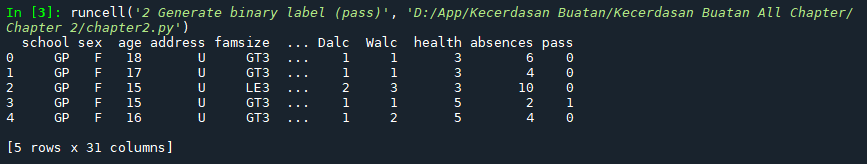
\includegraphics[scale=0.5]{figures/chapter2/2.PNG}
\end{figure}

\item
\begin{verbatim}
	# use one-hot encoding on categorical columns
	d = pd.get_dummies(d, columns=['sex', 'school', 'address', 
									'famsize', 
									'Pstatus', 'Mjob', 'Fjob', 
	                               'reason', 'guardian', 'schoolsup', 
								   'famsup', 'paid', 'activities',
	                               'nursery', 'higher', 'internet', 
									'romantic'])
	d.head()
\end{verbatim}
\newline Output: 
\begin{figure}[!htbp]
	\centering
	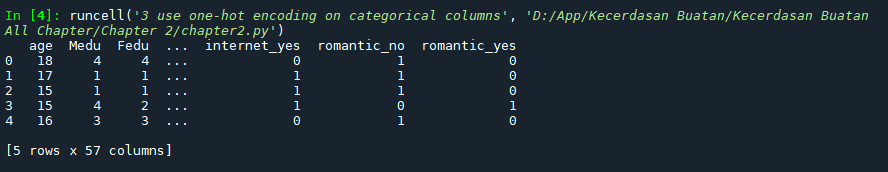
\includegraphics[scale=0.5]{figures/chapter2/3.PNG}
\end{figure}

\item
\begin{verbatim}
	# shuffle rows
	d = d.sample(frac=1)
	# split training and testing data
	d_train = d[:500]
	d_test = d[500:]

	d_train_att = d_train.drop(['pass'], axis=1)
	d_train_pass = d_train['pass']

	d_test_att = d_test.drop(['pass'], axis=1)
	d_test_pass = d_test['pass']

	d_att = d.drop(['pass'], axis=1)
	d_pass = d['pass']

	# number of passing students in whole dataset:
	import numpy as np
	print("Passing: %d out of %d (%.2f%%)" % (np.sum(d_pass), len(d_pass), 
	       100*float(np.sum(d_pass)) / len(d_pass)))
\end{verbatim}
\newline Output: 
\begin{figure}[!htbp]
	\centering
	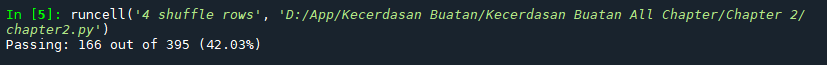
\includegraphics[scale=0.5]{figures/chapter2/4.PNG}
\end{figure}

\item 
\begin{verbatim}
	# fit a decision tree
	from sklearn import tree
	t = tree.DecisionTreeClassifier(criterion="entropy", max_depth=5)
	t = t.fit(d_train_att, d_train_pass)
\end{verbatim}
\newline Output: 
\begin{figure}[!htbp]
	\centering
	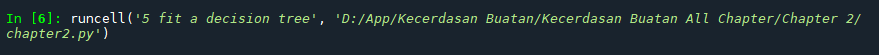
\includegraphics[scale=0.5]{figures/chapter2/5.PNG}
\end{figure}

\item
\begin{verbatim}
	# visualize tree
	import graphviz
	dot_data = tree.export_graphviz(t, out_file=None, label="all", 
									impurity=False, proportion=True,
	                                feature_names=list(d_train_att), 
									class_names=["fail", "pass"], 
	                                filled=True, rounded=True)
	graph = graphviz.Source(dot_data)
	graph
\end{verbatim}
\newline Output: 
\begin{figure}[!htbp]
	\centering
	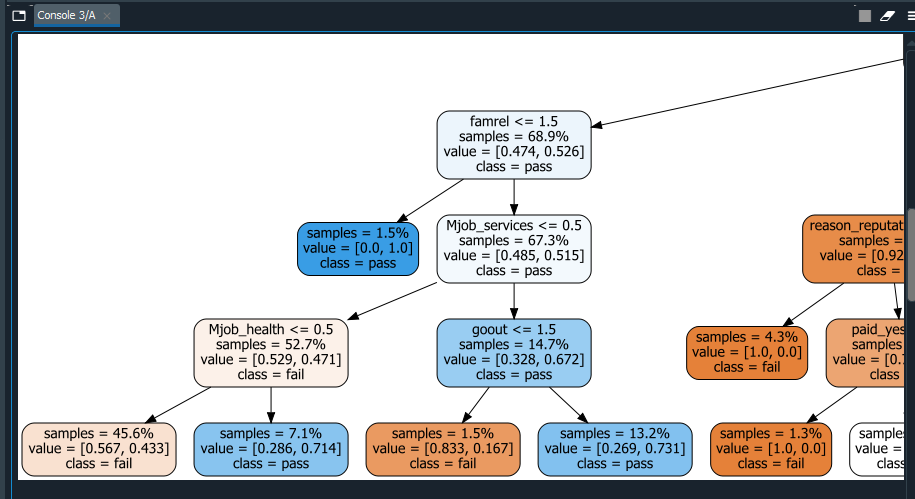
\includegraphics[scale=0.5]{figures/chapter2/6.PNG}
\end{figure}

\item
\begin{verbatim}
	# save tree
	tree.export_graphviz(t, out_file="student-performance.dot", 
						 label="all", impurity=False, 
						 proportion=True,
	                     feature_names=list(d_train_att), 
	                     class_names=["fail", "pass"], 
	                     filled=True, rounded=True)
\end{verbatim}
\newline Output: 
\begin{figure}[!htbp]
	\centering
	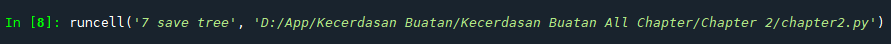
\includegraphics[scale=0.5]{figures/chapter2/7.PNG}
\end{figure}

\item
\begin{verbatim}
	t.score(d_test_att, d_test_pass)
\end{verbatim}
\newline Output: 
\begin{figure}[!htbp]
	\centering
	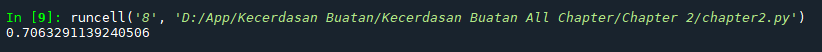
\includegraphics[scale=0.5]{figures/chapter2/8.PNG}
\end{figure}

\item
\begin{verbatim}
	from sklearn.model_selection import cross_val_score
	scores = cross_val_score(t, d_att, d_pass, cv=5)
	# show average score and +/- two standard deviations away 
	#(covering 95% of scores)
	print("Accuracy: %0.2f (+/- %0.2f)" % (scores.mean(), scores.std() * 2))
\end{verbatim}
\newline Output: 
\begin{figure}[!htbp]
	\centering
	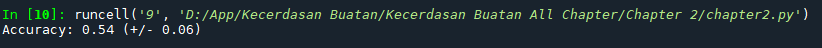
\includegraphics[scale=0.5]{figures/chapter2/9.PNG}
\end{figure}

\item 
\begin{verbatim}
	for max_depth in range(1, 20):
	    t = tree.DecisionTreeClassifier(criterion="entropy", 
			max_depth=max_depth)
	    scores = cross_val_score(t, d_att, d_pass, cv=5)
	    print("Max depth: %d, Accuracy: %0.2f (+/- %0.2f)" % 
				(max_depth, scores.mean(), scores.std() * 2)
			 )
\end{verbatim}
\newline Output: 
\newpage
\begin{figure}[!htbp]
	\centering
	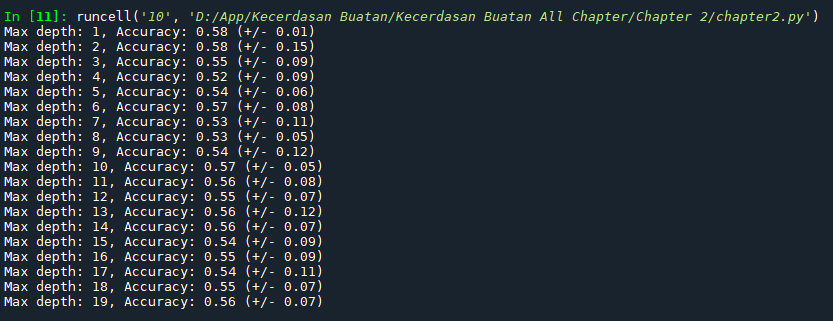
\includegraphics[scale=0.5]{figures/chapter2/10.PNG}
\end{figure}

\item
\begin{verbatim}
	depth_acc = np.empty((19,3), float)
	i = 0
	for max_depth in range(1, 20):
	    t = tree.DecisionTreeClassifier(criterion="entropy", 
			max_depth=max_depth)
	    scores = cross_val_score(t, d_att, d_pass, cv=5)
	    depth_acc[i,0] = max_depth
	    depth_acc[i,1] = scores.mean()
	    depth_acc[i,2] = scores.std() * 2
	    i += 1

	depth_acc
\end{verbatim}
\newline Output: 
\begin{figure}[!htbp]
	\centering
	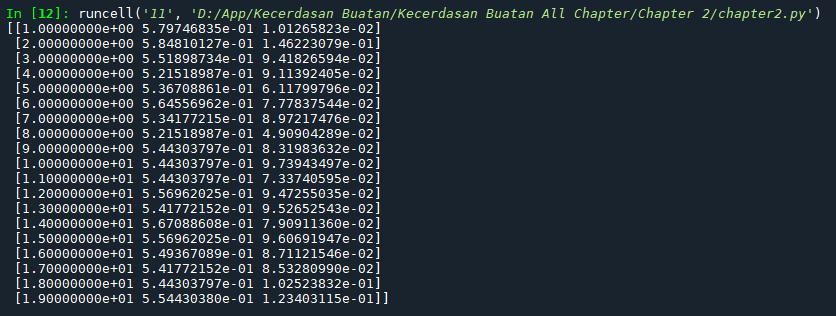
\includegraphics[scale=0.5]{figures/chapter2/11.PNG}
\end{figure}

\item 
\begin{verbatim}
	import matplotlib.pyplot as plt
	fig, ax = plt.subplots()
	ax.errorbar(depth_acc[:,0], depth_acc[:,1], yerr=depth_acc[:,2])
	plt.show()
\end{verbatim}
\newline Output: 
\begin{figure}[!htbp]
	\centering
	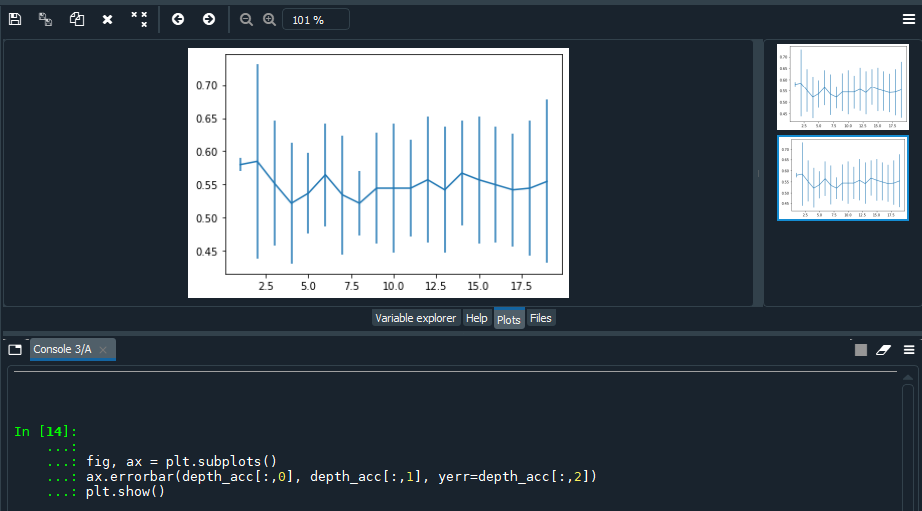
\includegraphics[scale=0.5]{figures/chapter2/12.PNG}
\end{figure}


\end{enumerate}

\newpage
\newpage
\section{Penanganan Error}
Dari percobaan yang dilakukan di atas, error yang kita dapatkan di dokumentasikan dan di selesaikan(nilai 5 hari kedua):

\begin{enumerate}
	\item Screenshot error.
	\begin{figure}[!htbp]
		\centering
		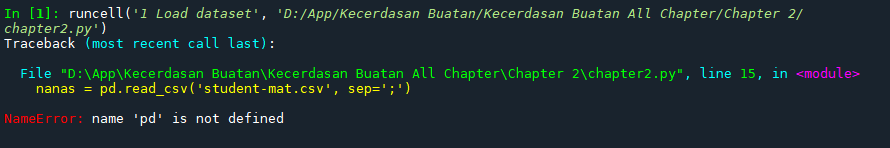
\includegraphics[scale=0.5]{figures/chapter2/13.PNG}
	\end{figure}
	
	\item Tuliskan kode eror dan jenis errornya.
	\begin{enumerate}
		\item NameError = name 'np' is not defined
	\end{enumerate}
	
	\item Solusi pemecahan masalah error tersebut.
	\begin{enumerate}
		\item NameError = Solusinya yaitu mengimport numpy dengan menginisialisaikannya sebagai np.
	\end{enumerate}
	
\end{enumerate}

